\chapter{Experimental Results}\label{ch:results}

\begin{flushright}
	\emph{\lq\lq A victory is twice itself when the achiever brings home full numbers.\rq\rq \\
		       \emph{Much ado about nothing}, Leonato, scene 1.}
\end{flushright}

\vspace{0.6cm}

In {\bf chapter \ref{ch:introduction}}, we introduced the concept of log-composition, whose computation is involved in some tools of medical imaging, as diffeomorphic registration and computation of the logarithm in the log-Euclidean framework. 
{\bf Chapter \ref{ch:tools}} is devoted to the introduction of the underpinning mathematical theory. Here three numerical methods for the computation of the log-composition are presented:
\begin{enumerate}
	\item Truncated BCH formula of degree $k=1,2,3$ - equation \ref{eq:bch_definition}.
	\item Taylor expansion - equation \ref{eq:taylor}.
	\item Parallel transport - equation \ref{eq:parallel_transport}.
\end{enumerate}
To evaluate their performance, two groups of transformations has been placed in a playground:
\begin{enumerate}
	\item The special euclidean group SE(2) - section \ref{se:rigid_body_transformations}
	\item The group diffeomorphisms corresponding to SVF - section \ref{se:svf}
\end{enumerate}
The first one is commonly used in medical image registration for rigid registration: it is a finite dimensional group and all of the computations involved in this research possess a closed formula. The second one is used in diffeomorphic image registration (section \ref{se:registration_framework}): it is an infinite dimensional group where no closed formulas are available. 
These are presented in {\bf chapter \ref{ch:spatial_transformations}} with respective numerical methods for their log-composition.\\
The computation of the logarithm appears to be an important piece in the jigsaw puzzle of the log-euclidean framework. The algorithm presented in 2008 in \cite{Bossa:08}, here called log-algorithm, can be an alternative to the usual inverse scaling and squaring algorithm initially proposed.  
The {\bf chapter \ref{ch:log_algorithm}} explains how the log-composition is involved in the log-algorithm and how each numerical methods for its computation implies a structural modification in the log-algorithm. The numerical methods tailored for the log-algorithm here presented are
\begin{enumerate}
	\item Truncated BCH formula of degree $k=1,2,3$ - equation \ref{eq:bossa_bch_strat}.
	\item Parallel transport - equation \ref{eq:bossa_parallel_strategy}.
	\item Symmetric parallel transport - equation \ref{eq:bossa_symmetric}.
\end{enumerate}

The performance of the log-composition with each of the presented methods, applied to the groups of transformations $SE(2)$ and diffeomorphisms parametrized by SVF, is evaluated over synthetic datasets.

% % % % % % % % % % % % % % % % % % % % % % % % % % % % % % % % % % % % % %
% % % % % % % % % % % % % % % % % % % % % % % % % % % % % % % % % % % % % % 
% % % % % % % % % % % % % % % % % % % % % % % % % % % % % % % % % % % % % % 
\section{Log-composition for $\mathfrak{se}(2)$}

% % % % % % % % % % % % % % % % % % % % % % % % % % % % % % % % % % % % % %
% % % % % % % % % % % % % % % % % % % % % % % % % % % % % % % % % % % % % % 
\subsection{Methods}

A set of $500$ transformations in $\mathfrak{se}(2)$ are sampled with a randomizer. Whereas the Frobenius norm of the matrix representation of $SE(2)$ is not proportional to the rotation angle $\theta$, in $\mathfrak{se}(2)$ it is
\begin{align*}
\euclideanMetric{(\theta,dt_{x},dt_{y})}_{\text{fro}} = \sqrt{2\theta^{2} + dt_{x}^2 + dt_{y}^2} 
\end{align*}




on with frobenius norm between $0.0$ and $1.0$


% % % % % % % % % % % % % % % % % % % % % % % % % % % % % % % % % % % % % %
% % % % % % % % % % % % % % % % % % % % % % % % % % % % % % % % % % % % % % 
\subsection{Results}









\begin{figure}[!ht]
	%\centering
	\hspace{-3cm}
	\includegraphics[scale=0.65]{figures/se2_four_BCH.png}
	\caption{comparisons between BCH methods. TODO}
	\label{fig:se2_four_BCH}
\end{figure}

\begin{figure}[!ht]
	%\centering
	\hspace{-2cm}
	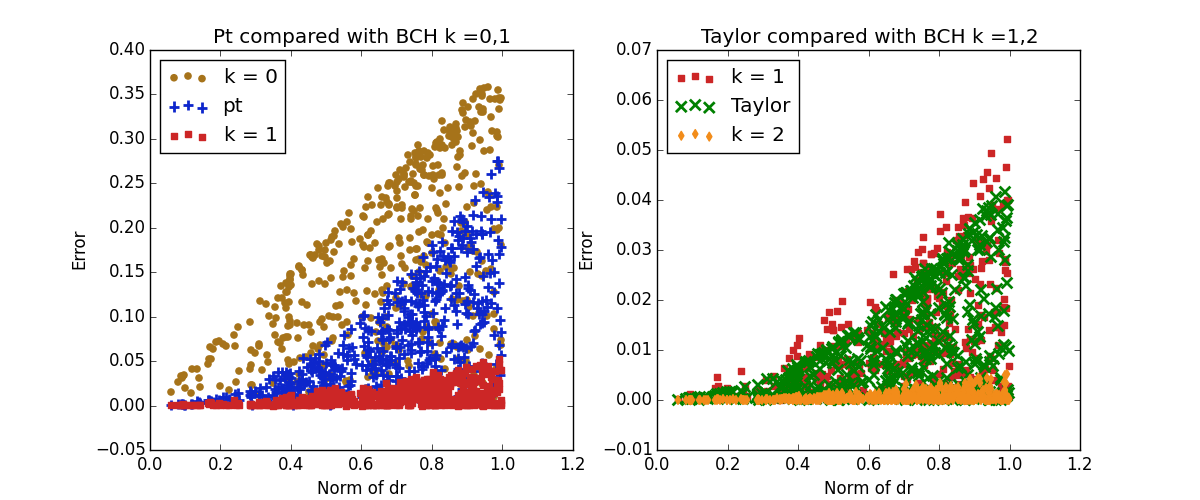
\includegraphics[scale=0.6]{figures/se2_pt_taylor.png}
	\caption{comparisons between Parallel Transport method and Taylor method. TODO}
	\label{fig:se2_pt_taylor}
\end{figure}


\begin{figure}[!ht]
	\hspace{-2cm}
	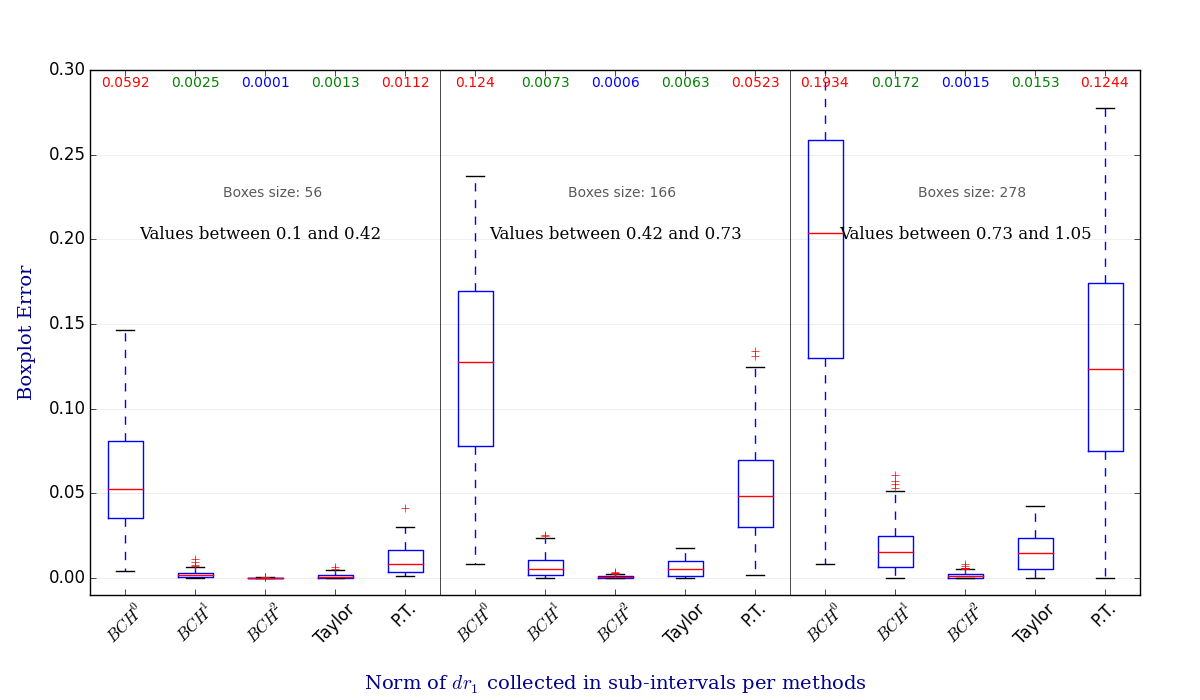
\includegraphics[scale=0.75]{figures/se2_boxplot.png}
	\caption{comparisons between all the methods. TODO}
	\label{fig:se2_boxplot}
\end{figure}


% % % % % % % % % % % % % % % % % % % % % % % % % % % % % % % % % % % % % %
% % % % % % % % % % % % % % % % % % % % % % % % % % % % % % % % % % % % % % 
\subsection{Empirical Evaluations of Computational Time}


% % % % % % % % % % % % % % % % % % % % % % % % % % % % % % % % % % % % % % 
% % % % % % % % % % % % % % % % % % % % % % % % % % % % % % % % % % % % % % 
\section{Log-composition for SVF}
Using a python software, we created synthetic random matrices in $\mathfrak{se}(2)$. We considered the difference between the log composition computed with the closed form \ref{eq:log_composition_se2_closed_form}. 
A sample of $500$ couples $(dr_0,dr_1)$ of elements in $\mathfrak{se}(2)$ are created, 


% % % % % % % % % % % % % % % % % % % % % % % % % % % % % % % % % % % % % %
% % % % % % % % % % % % % % % % % % % % % % % % % % % % % % % % % % % % % % 
\subsection{Methods}

% % % % % % % % % % % % % % % % % % % % % % % % % % % % % % % % % % % % % %
% % % % % % % % % % % % % % % % % % % % % % % % % % % % % % % % % % % % % % 
\subsection{Results}

% % % % % % % % % % % % % % % % % % % % % % % % % % % % % % % % % % % % % %
% % % % % % % % % % % % % % % % % % % % % % % % % % % % % % % % % % % % % % 
\subsection{Empirical Evaluations of Computational Time}

% % % % % % % % % % % % % % % % % % % % % % % % % % % % % % % % % % % % % %
% % % % % % % % % % % % % % % % % % % % % % % % % % % % % % % % % % % % % % 
% % % % % % % % % % % % % % % % % % % % % % % % % % % % % % % % % % % % % % 
\section{Log-computation Algorithm for SVF}

% % % % % % % % % % % % % % % % % % % % % % % % % % % % % % % % % % % % % %
% % % % % % % % % % % % % % % % % % % % % % % % % % % % % % % % % % % % % % 
\subsection{Methods}

% % % % % % % % % % % % % % % % % % % % % % % % % % % % % % % % % % % % % %
% % % % % % % % % % % % % % % % % % % % % % % % % % % % % % % % % % % % % % 
\subsection{Results}


% % % % % % % % % % % % % % % % % % % % % % % % % % % % % % % % % % % % % %
% % % % % % % % % % % % % % % % % % % % % % % % % % % % % % % % % % % % % % 
\subsection{Empirical Evaluations of Computational Time}


% % % % % % % % % % % % % % % % % % % % % % % % % % % % % % % % % % % % % %
% % % % % % % % % % % % % % % % % % % % % % % % % % % % % % % % % % % % % %
% % % % % % % % % % % % % % % % % % % % % % % % % % % % % % % % % % % % % % 
\section{Conclusion and Further Research}\label{ch:conclusions}


Considering only the results, this one-year research can be considered much ado about nothing, but...\\
Computational time...!